\newpage
\flushleft
\section*{Appendix A - 2D Enclosed Flow Results} 
\label{sec: appendix_a}

\addcontentsline{toc}{section}{Appendix A - 2D Enclosed Flow Results}

\begin{figure}[!ht]
    \centering
    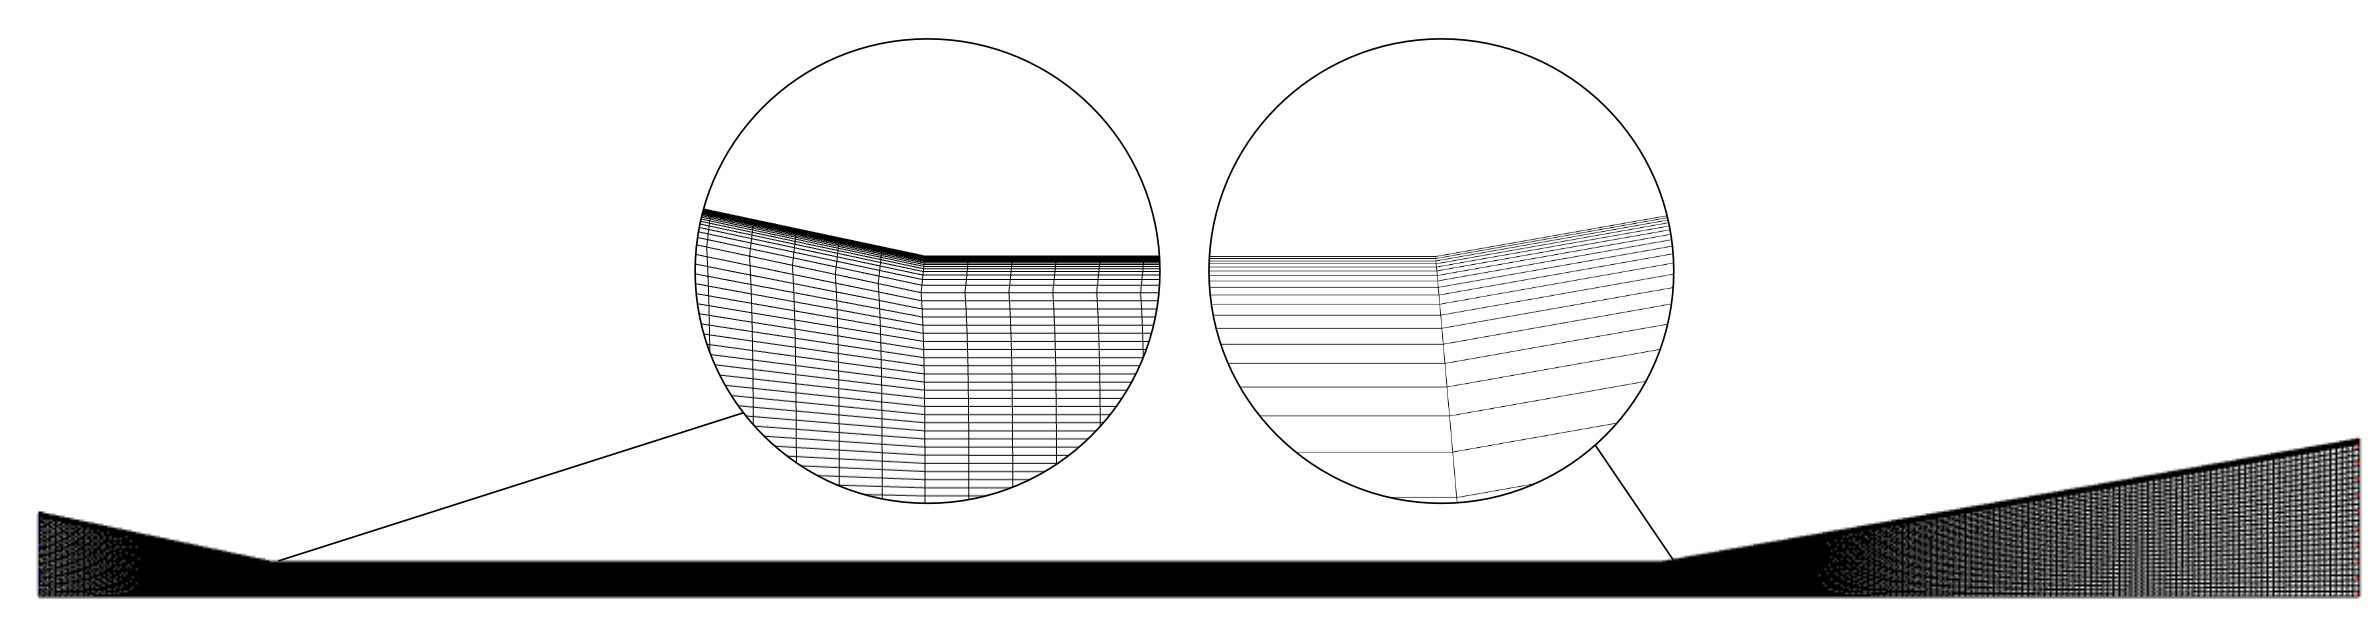
\includegraphics[scale = 0.7]{Figures/2D_EN/2D_EN_MESH_COMPLETE.png}
    \caption{2D enclosed flow mesh consist of quadrilateral mesh with 20 inflation layer Y$^+$=1 generated} 
    \label{fig:2D_EN_MESH}
\end{figure}

\begin{center}
  \begin{figure}[!ht]
    \centering
    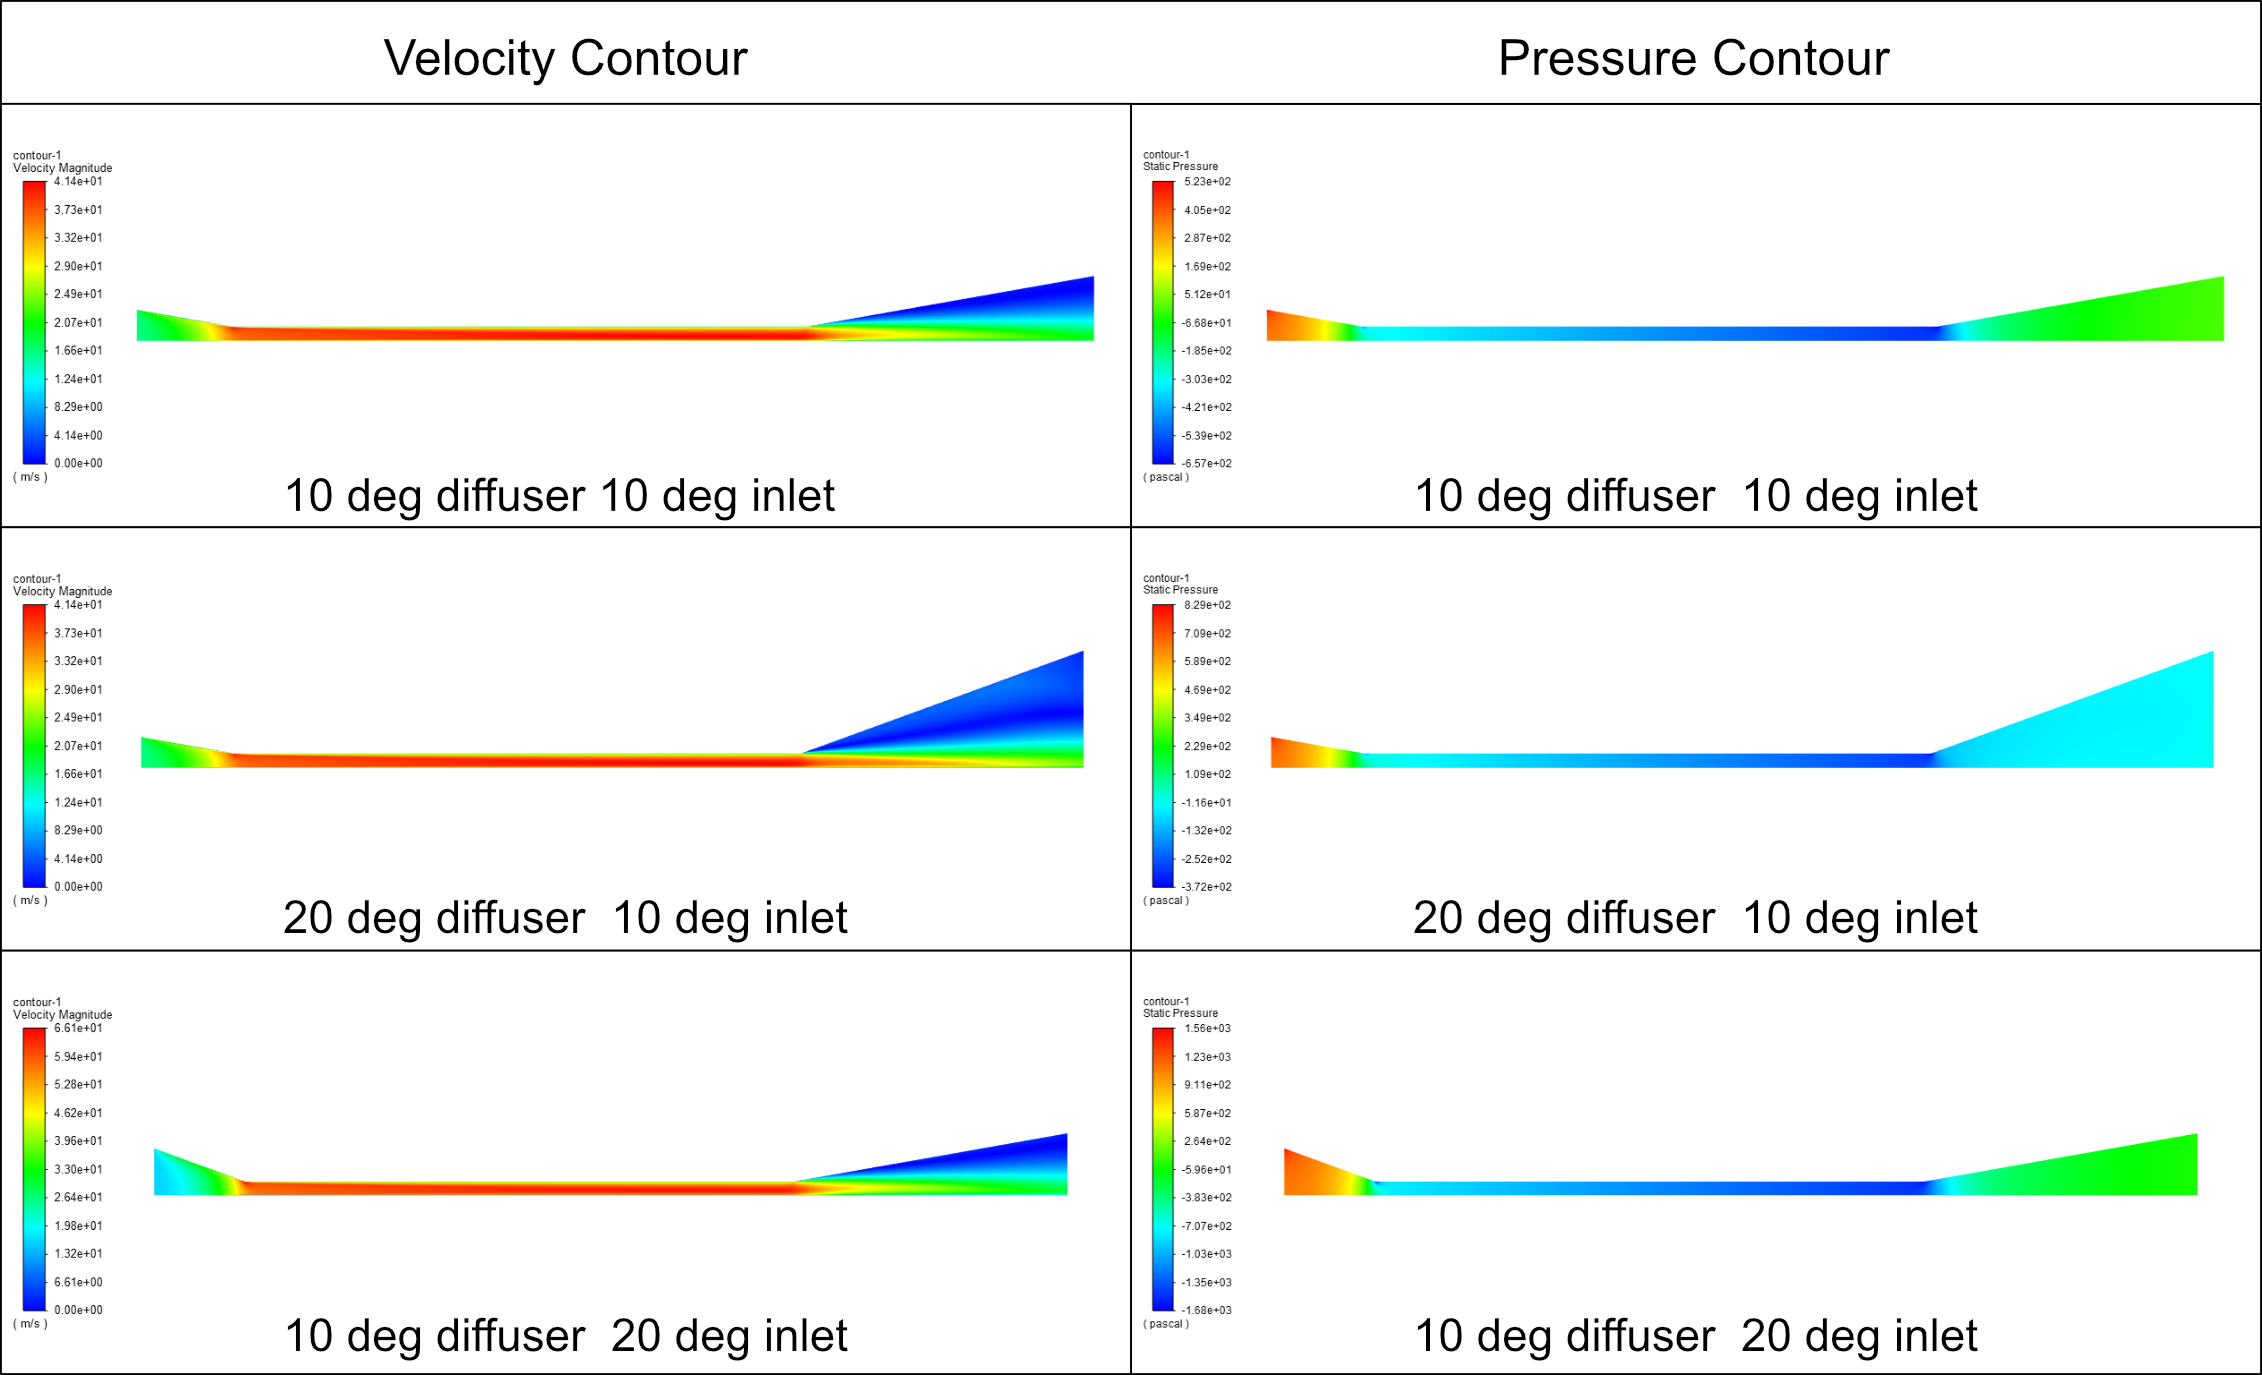
\includegraphics[scale=0.8]{Figures/2D_EN/COMPILE_APPENDIX_A_PRESSVELO.png}
    \caption{Velocity (left) and (right) pressure contour of the undertray in three states: baseline (top), maximum diffuser angle (middle), and maximum inlet angle (bottom).}
    \label{fig:compile_2D_EN_pressure_velocity}
\end{figure}

\begin{figure}[!ht]
    \centering
    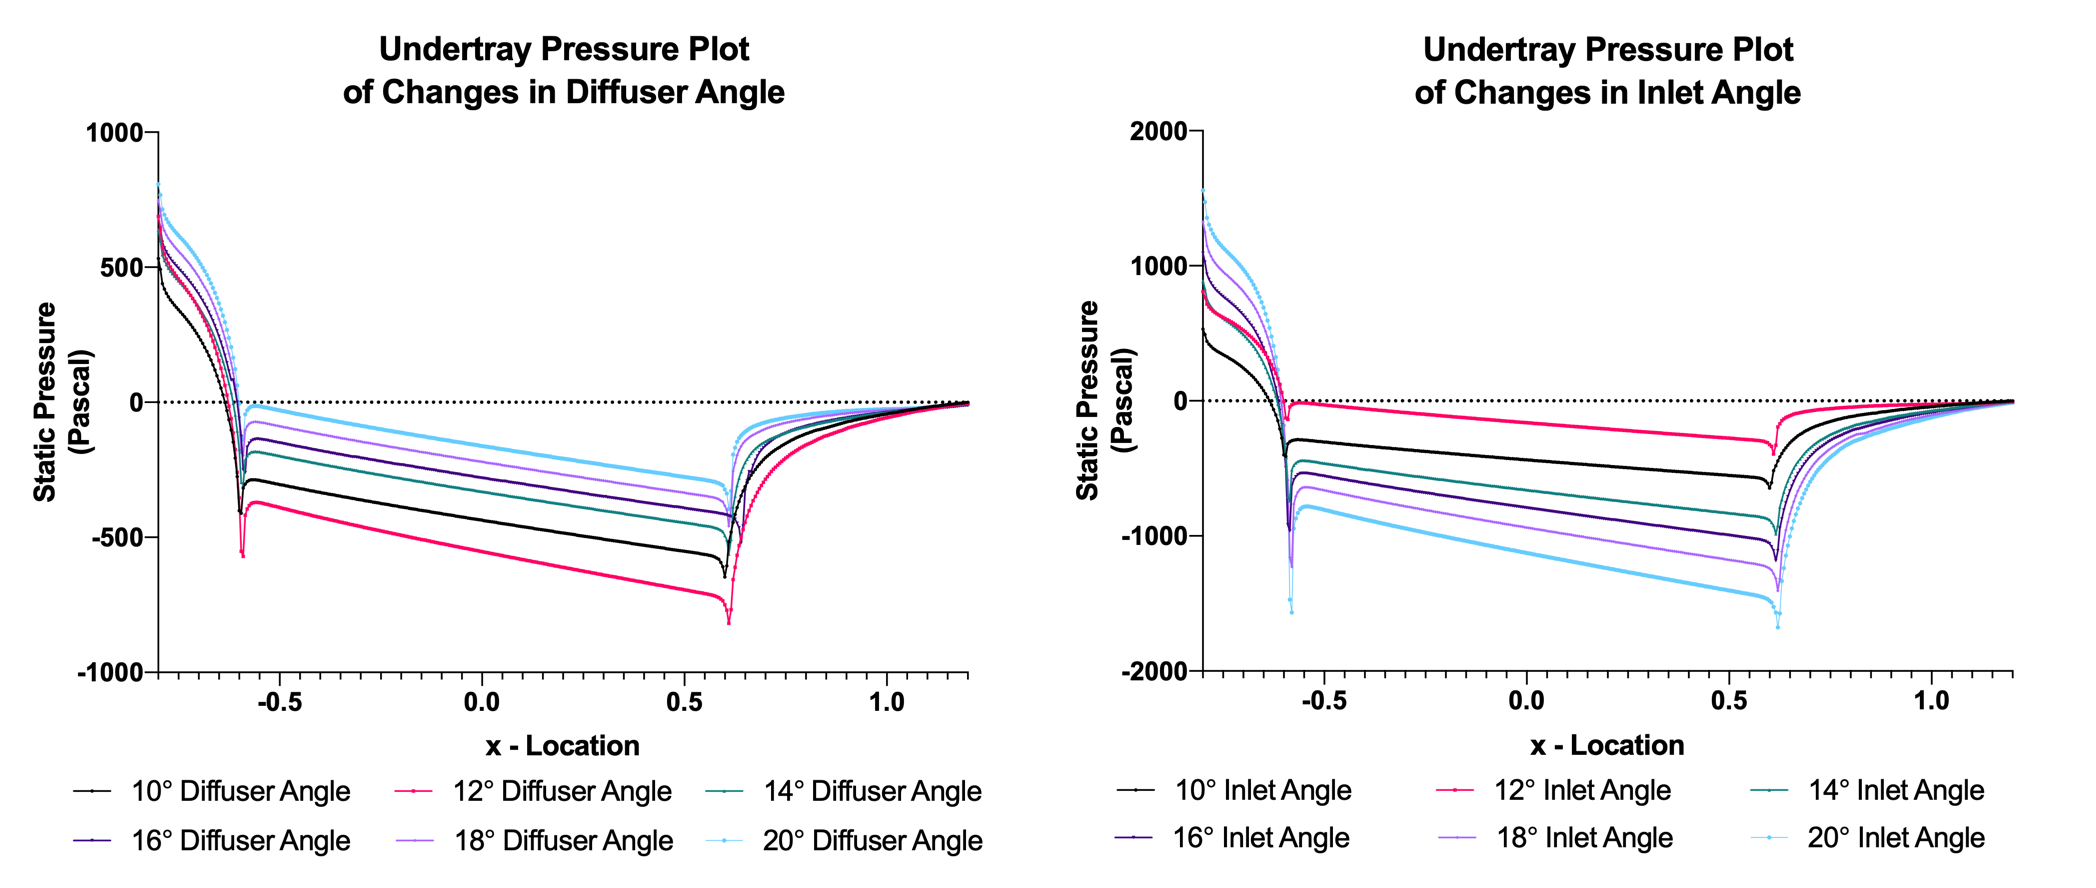
\includegraphics[height = 6.5cm]{Figures/2D_EN/2D_EN_UT_Presspdf.png}
    \caption{Static pressure plot of undertray's wall with changes in diffuser (left) and inlet (right) angle.}
    \label{fig:pressure_plot_2D_EN}
\end{figure}

\begin{figure}[!ht]
    \centering
    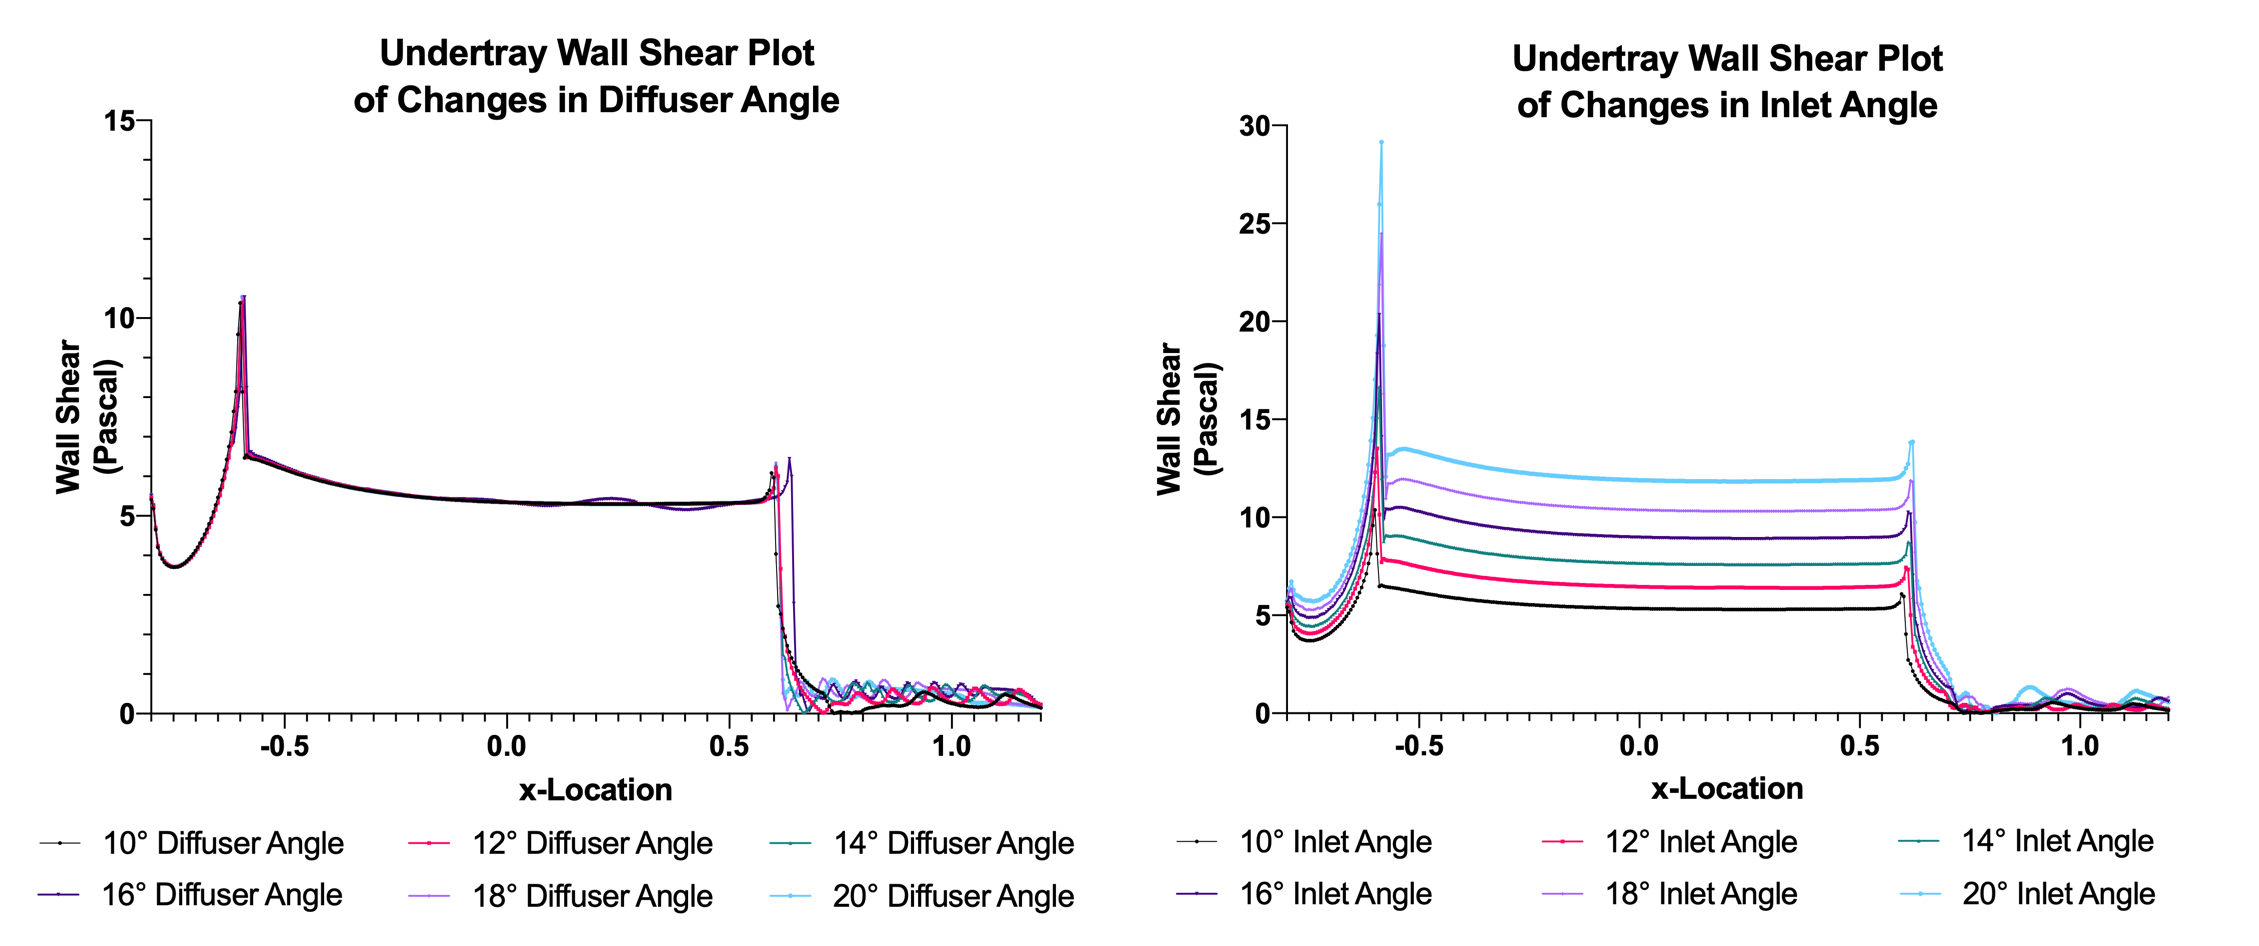
\includegraphics[height = 6.5cm]{Figures/2D_EN/2D_EN_UT_WShear.png}
    \caption{Wall Shear plot of undertray's wall with changes in diffuser (left) and inlet (right) angle.}
    \label{fig:wall_shear_plot_2D_EN}
\end{figure}  
\end{center}

